% Activation patching figure for the Literature Survey.
% Same style as animatediff_arch.tex and ldm_pipeline.tex; drawn at the report's \textwidth (16.5cm).
% Build: pdflatex patching_diagram.tex  ->  patching_diagram.pdf
\documentclass[tikz,border=1pt]{standalone}
\usepackage{amsmath,amssymb}
\usetikzlibrary{positioning,arrows.meta,calc,fit,backgrounds}

\definecolor{frzF}{HTML}{E9E9E9}\definecolor{frzD}{HTML}{8C8C8C}
\definecolor{trnF}{HTML}{FBD9B5}\definecolor{trnD}{HTML}{C8661B}
\definecolor{perF}{HTML}{CFE0F3}\definecolor{perD}{HTML}{3F6FA8}

\tikzset{
  >={Stealth[length=1.6mm]},
  font=\sffamily\scriptsize,
  flow/.style={->, draw=black!60},
  st/.style={circle, draw=frzD, fill=white, minimum size=0.24cm, inner sep=0pt},
  stc/.style={st, fill=perF, draw=perD},
  stx/.style={st, fill=frzF, draw=frzD},
  stp/.style={st, fill=trnF, draw=trnD, line width=0.9pt},
  copy/.style={->, draw=trnD, very thick},
  lbl/.style={font=\sffamily\scriptsize, text=black!80},
  ttl/.style={font=\sffamily\footnotesize\bfseries},
  ub/.style={draw=frzD, fill=frzF, minimum width=0.62cm, minimum height=0.50cm, inner sep=0pt, rounded corners=1pt},
}

% a grid of hidden states: 5 tokens x 4 layers, lower-left at (#1,#2); #3 = style; #4 = name prefix
\newcommand{\states}[4]{%
  \foreach \i in {1,...,5}{\foreach \l in {1,...,4}{%
    \node[#3] (#4-\i-\l) at ($(#1,#2)+(\i*0.52,\l*0.36)$) {};}}}

\begin{document}
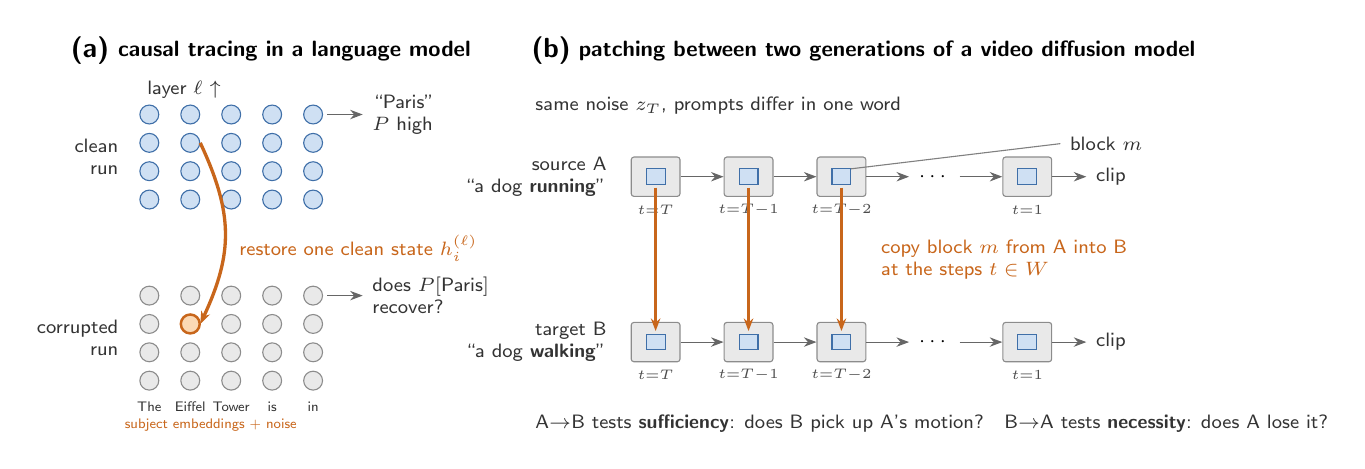
\begin{tikzpicture}

% ---------------- (a) causal tracing in a language model ----------------
\node[font=\sffamily\normalsize\bfseries, anchor=west] at (-0.05,4.55) {(a)};
\node[ttl, anchor=west] at (0.55,4.55) {causal tracing in a language model};

% clean run
\states{0.55}{2.30}{stc}{c}
\node[lbl, anchor=east, align=right] at (0.80,3.20) {clean\\run};
% corrupted run, subject tokens noised at the input
\states{0.55}{0.00}{stx}{x}
\node[lbl, anchor=east, align=right] at (0.80,0.90) {corrupted\\run};
% restored state
\node[stp] at (x-2-3) {};
\draw[copy] (c-2-3.east) .. controls +(0.42,-0.9) and +(0.42,0.9) .. (x-2-3.east);
\node[lbl, text=trnD, anchor=west] at ($(c-3-1)+(-0.02,-0.62)$) {restore one clean state $h_i^{(\ell)}$};

% tokens
\foreach \i/\w in {1/The,2/Eiffel,3/Tower,4/is,5/in}{%
  \node[lbl, font=\sffamily\tiny] at ($(x-\i-1)+(0,-0.33)$) {\w};}
\node[font=\sffamily\tiny, text=trnD] at ($(x-2-1)!0.5!(x-3-1)+(0,-0.56)$) {subject embeddings + noise};
\node[lbl, anchor=west] at ($(c-1-4)+(-0.15,0.32)$) {layer $\ell$ $\uparrow$};

% outputs
\draw[flow] ($(c-5-4)+(0.18,0)$) -- ++(0.45,0) node[right, lbl, align=left] {``Paris''\\$P$ high};
\draw[flow] ($(x-5-4)+(0.18,0)$) -- ++(0.45,0) node[right, lbl, align=left] {does $P[\text{Paris}]$\\recover?};

% ---------------- (b) the same idea across denoising steps ----------------
\begin{scope}[shift={(5.85,0)}]
  \node[font=\sffamily\normalsize\bfseries, anchor=west] at (-0.05,4.55) {(b)};
  \node[ttl, anchor=west] at (0.55,4.55) {patching between two generations of a video diffusion model};

  \node[lbl, anchor=west] at (0.0,3.85) {same noise $z_T$, prompts differ in one word};
  % source and target trajectories
  \foreach \r/\y/\nm/\p in {A/2.95/source A/{``a dog \textbf{running}''}, B/0.85/target B/{``a dog \textbf{walking}''}}{%
    \node[lbl, anchor=east, align=right] at (1.15,\y) {\nm\\\p};
    \foreach \k/\t in {0/T,1/T{-}1,2/T{-}2,4/1}{%
      \node[ub] (\r\k) at ($(1.65,\y)+(\k*1.18,0)$) {};
      \node[font=\sffamily\tiny, text=black!70] at ($(\r\k)+(0,-0.42)$) {$t{=}\t$};}
    \node[minimum width=0.62cm, minimum height=0.50cm] (\r3) at ($(1.65,\y)+(3*1.18,0)$) {$\cdots$};
    \foreach \k in {0,1,2,4}{\fill[perF, draw=perD] ($(\r\k)+(-0.12,-0.10)$) rectangle ++(0.24,0.20);}
    \foreach \a/\b in {0/1,1/2,2/3,3/4}{\draw[flow] (\r\a) -- (\r\b);}
    \draw[flow] (\r4) -- ++(0.75,0) node[right, lbl] (\r out) {clip};}

  % copies at block m in the step window W
  \foreach \k in {0,1,2}{\draw[copy] ($(A\k)+(0,-0.14)$) -- ($(B\k)+(0,0.14)$);}
  \node[lbl, text=trnD, align=left, anchor=west] at ($(A2)+(0.38,-1.05)$)
    {copy block $m$ from A into B\\at the steps $t \in W$};

  % reading the result
  \node[lbl, align=left, anchor=north west] at (0.0,0.05)
    {A$\to$B tests \textbf{sufficiency}: does B pick up A's motion?\quad
     B$\to$A tests \textbf{necessity}: does A lose it?};
  \node[lbl, anchor=west] at ($(A4)+(0.42,0.42)$) {block $m$};
  \draw[black!50] ($(A4)+(0.42,0.42)$) -- ($(A2)+(0.12,0.10)$);
\end{scope}

\end{tikzpicture}
\end{document}
